\documentclass{article}
\author{Otetc pitona}
\usepackage[russian]{babel}
\usepackage[utf8]{inputenc}
\usepackage{geometry}
\usepackage[12pt]{extsizes}
\usepackage{setspace}
\usepackage{amsmath}
\usepackage{tikz}  
\usetikzlibrary{shapes.geometric}
\usepackage{verbatim}
\usetikzlibrary{graphs}
\usetikzlibrary{tikzmark,overlay-beamer-styles}
\usetikzlibrary{arrows}
\geometry{
	a4paper,
	top=3mm, 
	right=4mm, 
	bottom=4mm, 
	left=4mm,
	head=-1mm
}
\tikzstyle{materia}=[draw, text width=6.0em, text centered,
minimum height=1.5em]
\tikzstyle{block} = [materia, text width=8em, minimum width=10em,
minimum height=3em, rounded corners]
\begin{document}
\begin{center}
	\textbf{МОСКОВСКИЙ АВИАЦИОННЫЙ ИНСТИТУТ}
	\\
	\textbf{(НАЦИОНАЛЬНЫЙ ИССЛЕДОВАТЕЛЬСКИЙ УНИВЕРСИТЕТ)}
	\\ 
	\textbf{ФАКУЛЬТЕТ ИНФОРМАЦИОННЫХ ТЕХНОЛОГИЙ И ПРИКЛАДНОЙ МАТЕМАТИКИ}
	\\ 
	\textbf{КАФЕДРА МАТЕМАТИЧЕСКОЙ КИБЕРНЕТИКИ}
\end{center}
\vspace{100mm}
\begin{center}
	\begin{Large}\textbf{КУРСОВАЯ РАБОТА}\end{Large}
	\vspace{5mm}
	\\
	\textbf{Пересчет прадеревьев ориентированного графа и их построение.}
\end{center}
\vspace{70mm}
\begin{large}
	\par
	\hspace{105mm}\textbf{Студент: Ершов С.Г.}
	\vspace{3mm}
	\par
	\hspace{105mm}\textbf{Группа 8О-103Б}
	\vspace{3mm}
	\par
	\hspace{105mm}\textbf{Преподаватель: Смерчинская С.О.}
	\vspace{3mm}
	\par
	\hspace{105mm}\textbf{Оценка:}
	\vspace{3mm}
	\par
	\hspace{105mm}\textbf{Дата:}
\end{large}
\newpage


\voffset = 8mm
\begin{flushleft}
	\begin{Large}
		\hspace{8mm}\textbf{Задание}
		\vspace{10mm}
		\\
		\hspace{8mm}\textbf{Вариант 8}
	\end{Large}
\end{flushleft}
\vspace{8mm}
\large
\hspace{8mm}\textbf{1.} Определить для орграфа, заданного матрицей смежности:
\vspace{5mm}
\\
\hspace*{50mm}
$A = 
\begin{pmatrix}
	0 & 0 & 1 & 1\\
	1 & 0 & 0 & 1\\
	0 & 0 & 0 & 0\\
	1 & 0 & 1 & 0\\
\end{pmatrix}$
\vspace{5mm}
\\
\hspace*{12mm} а) матрицу односторонней связности;
\\
\hspace*{12mm} б) матрицу сильной связности;
\\
\hspace*{12mm} в) компоненты сильной связности;
\\
\hspace*{12mm} г) матрицу контуров;
\\
\hspace*{12mm} д) изображение графа и компонент сильной связности;
\\
\\
\hspace*{8mm}\textbf{2.} Используя алгоритм Терри, определить замкнутый маршрут, проходящий ровно
\\
\hspace*{12mm} по два раза (по одному в каждом направлении) через каждое ребро графа.
\vspace{5mm}
\\

\begin{tikzpicture}
	[node distance={30mm}, thick, main/.style = {draw, circle}]
	\hspace*{50mm}\node[main] (1) {$2$}; 
	\node[main] (2) [below of=1] {$1$};
	\node[main] (3) [right of=1] {$3$};
	\node[main] (5) [below of=3] {$5$};
    \node[main] (4) [right of=5] {$4$};
    \draw(3) -- (2);
    \draw(1) -- (3);
    \draw(1) -- (5);
    \draw(1) -- (2);
    \draw(5) -- (4);
    \draw(5) -- (3);
    \draw(4) -- (3);
    \draw (2) -- (5);
\end{tikzpicture} 
\\
\\
\hspace*{8mm}\textbf{3.} Используя алгоритм “фронта волны”, найти все минимальные пути из первой
\\
\hspace*{12mm} вершины в последнюю орграфа, заданного матрицей смежности.
\vspace{5mm}
\\
\hspace*{40mm}
$A = 
\begin{pmatrix}
	0 & 0 & 0 & 1 & 0 & 0 & 1 & 0\\
	1 & 0 & 1 & 0 & 1 & 0 & 1 & 0\\
	0 & 1 & 0 & 1 & 0 & 1 & 0 & 1\\
	1 & 0 & 0 & 0 & 0 & 1 & 1 & 0\\
	1 & 0 & 1 & 1 & 0 & 0 & 1 & 0\\
	0 & 1 & 0 & 1 & 1 & 0 & 1 & 0\\
	0 & 0 & 0 & 1 & 0 & 1 & 0 & 0\\
	1 & 1 & 1 & 1 & 0 & 0 & 0 & 0\\
\end{pmatrix}$


\newpage
\hoffset=2mm
\textbf{4.} Используя алгоритм Форда, найти минимальные пути из первой вершины во все
\\ \hspace*{10mm} достижимые вершины в нагруженном графе, заданном матрицей длин дуг.
\vspace{5mm}
\\
\hspace*{40mm}
$A = 
\begin{pmatrix}
	\infty & 5 & 2 & 7 & \infty & \infty & \infty & \infty \\
	3 & \infty & 2 & 3 & \infty  & \infty & \infty & \infty \\
	\infty & 2 & \infty & \infty & 3 & \infty & \infty & \infty \\
	5 & \infty & \infty & \infty & 1 & 4 & \infty & 9 \\
	4 & \infty & \infty & 1 & \infty & \infty & 2 & \infty \\
	6 & \infty & \infty & \infty & \infty & \infty & 4 & 5 \\
	\infty & \infty & \infty & \infty & \infty & 4 & \infty & 9 \\
    8 & \infty & \infty & \infty & \infty & \infty & 15 & \infty
\end{pmatrix}$
\vspace{5mm}
\\
\hspace*{4mm} \textbf{5.}  Найти остовное дерево с минимальной суммой длин входящих в него ребер.
\vspace{5mm}
\\
\begin{tikzpicture}
	[node distance={20mm}, thick, main/.style = {draw, circle}]
	\hspace*{50mm}
	\node[main] (1) {$$};
	\node[main] (2) [right of = 1] {$$};
	\node[main] (3) [right of = 2]{$$};
	\node[main] (4) [right of = 3]{$$};
	\node[main] (5) [below of = 1]{$$};
	\node[main] (6) [below of = 2]{$$};
	\node[main] (7) [below of = 3] {$$};
	\node[main] (8) [below of = 4] {$$};
	\node[main] (9) [below of = 5] {$$};
	\node[main] (10) [below of = 6] {$$};
	\node[main] (11) [below of = 7] {$$};
	\node[main] (12) [below of = 8] {$$};
	\draw (1) -- node[above] {3} (2);
	\draw (2) -- node[above] {2} (3);
	\draw (3) -- node[above] {6} (4);
	\draw (1) -- node[left] {1} (5);
	\draw (2) -- node[left] {5} (6);
	\draw (3) -- node[left] {5} (7);
	\draw (4) -- node[right] {1} (8);
	\draw (5) -- node[above] {5} (6);
	\draw (6) -- node[above] {9} (7);
	\draw (7) -- node[above] {7} (8);
	\draw (5) -- node[left] {6} (9);
	\draw (6) -- node[left] {5} (10);
	\draw (7) -- node[left] {5} (11);
	\draw (8) -- node[right] {3} (12);
	\draw (9) -- node[below] {4} (10);
	\draw (10) -- node[below] {3} (11);
	\draw (11) -- node[below] {2} (12);
\end{tikzpicture} 
\vspace{5mm}
\\
\hspace*{4mm} \textbf{6.}  Пусть каждому ребру неориентированного графа соответствует некоторый
\\ \hspace*{12mm}элемент электрической цепи. Составить линейно независимые системы
\\ \hspace*{12mm}уравнений Кирхгофа для токов и напряжений. Пусть первому и пятому ребру
\\ \hspace*{12mm}соответствуют источники тока с ЭДС $E1$ и $E2$, а остальные элементы являются
\\ \hspace*{10mm} сопротивлениями.  Используя закон Ома, и, предполагая внутренние
\\ \hspace*{12mm}сопротивления источников тока равными нулю, получить систему уравнений для
\\ \hspace*{10mm} токов.
\vspace{5mm}
\\
\begin{tikzpicture}
	[node distance={40mm}, thick, main/.style = {draw, circle}]
	\hspace*{50mm}
	\node[main] (1) {$$};
	\node[main] (2) [right of = 1] {$$};
	\node[main] (3) [below of = 1]{$$};
	\node[main] (4) [right of = 3]{$$};
	\node[main] (5) [right of = 4]{$$};
    
    \draw (1) -- node[above] {$q_2$} (2);
    \draw (1) -- node[left = 1] {$q_1$} (3);
    \draw (2) -- node[above] {$q_6$} (5);
   \draw (3) to [out=10,in=245,looseness=0.5] node[below = 11mm, left = 3mm] {$q_3$} (2);
   \draw (5) -- node[left = 40, above = 20] {$q_4$} (1);
   \draw (5) to [out=270,in=270,looseness=0.5] node[below = 2] {$q_5$} (3);
    \draw (2) -- node[below = 30, right = 1] {$q_7$} (4);
    \draw (5) to [out=245, in=330, looseness=0.5] node[below=1] {$q_9$} (4);
    \draw (4) to [out=35, in=170, looseness=0.5] node[below=1] {$q_8$} (5);
    \draw (3) -- node[below] {$q_{10}$} (4);
    
\end{tikzpicture} 

\newpage
\noindent
\hspace*{4mm} \textbf{7.} Построить максимальный поток по транспортной сети.
\vspace{5mm}
\\
\begin{tikzpicture}
	[node distance={20mm}, thick, main/.style = {draw, circle}]
	\hspace*{30mm}
	\node[main] (1) {$1$};
	\node[main] (2) [above right of = 1, above = 20pt, right = 3pt] {$2$};
	\node[main] (3) [above right of = 2, above = -5mm, right = 40pt, node distance={20mm}]{$3$};
	\node[main] (4) [below right of = 3, below = -5mm, right = 40pt]{$4$};
	\node[main] (5) [right of = 1, node distance={45mm}]{$5$};
	\node[main] (6) [right of = 5, node distance={65mm}]{$9$};
	\node[main] (7) [below right of = 1, below = 20pt, right = 3pt] {$6$};
	\node[main] (8) [below right of = 7, below = -5mm, right = 40pt, node distance={20mm}]{$7$};
	\node[main] (9) [above right of = 8, above= -5mm, right = 40pt]{$4$};
	\draw[->] (1) -- node[above] {3} (2);
	\draw[->] (2) -- node[above] {3} (3);
	\draw[->] (3) -- node[above] {10} (4);
	\draw[->] (4) -- node[above] {12} (6);
	\draw[->] (1) to [out=0,in=230,looseness=0.5] node[above = -2mm, left = 5mm] {11} (3);
	\draw[->] (1) -- node[above = 3mm, right=5mm] {7} (5);
	\draw[->] (5) -- node[above] {6} (6);
	\draw[->] (1) -- node[below] {4} (7);
	\draw[->] (7) -- node[below] {4} (8);
	\draw[->] (8) -- node[below] {9} (9);
	\draw[->] (9) -- node[below] {12} (6);
	\draw[->] (1) to [out=0,in=130,looseness=0.5] node[below = -2mm, left = 5mm] {9} (8);
	\draw[->] (2) -- node[above = 6mm, left = 1mm] {2} (5);
	\draw[->] (5) -- node[above] {3} (4);
	\draw[->] (7) -- node[above] {3} (5);
	\draw[->] (5) -- node[above] {2} (9);
\end{tikzpicture} 
\vspace{5mm}
\\
\hspace*{4mm} \textbf{8.} Пересчет прадеревьев ориентированного графа и их построение. 
\\
\hspace*{11mm}1. Изучить алгоритм.
\\
\hspace*{11mm}2. Составить программу алгоритма.
\\
\hspace*{11mm}3. Отладить тестовые примеры.
\\
\hspace*{11mm}4. Провести оценку сложности алгоритма.
\\
\hspace*{11mm}5. Составить прикладную задачу, для решения которой используется данный алгоритм.


\newpage
\large
\begin{center}
		\textbf{Задание №1}
\end{center}
\par
а) \textbf{Способ №1}
\vspace{5mm}
\par \hspace{8mm} $A = 
\begin{pmatrix}
	0 & 0 & 1 & 1\\
	1 & 0 & 0 & 1\\
	0 & 0 & 0 & 0\\
	1 & 0 & 1 & 0\\
\end{pmatrix}$
\vspace{5mm}
\par

\hspace{8mm} $A^2 = 
\begin{pmatrix}
	0 & 0 & 1 & 1\\
	1 & 0 & 0 & 1\\
	0 & 0 & 0 & 0\\
	1 & 0 & 1 & 0\\
\end{pmatrix}$
$\begin{pmatrix}
	0 & 0 & 1 & 1\\
	1 & 0 & 0 & 1\\
	0 & 0 & 0 & 0\\
	1 & 0 & 1 & 0\\
\end{pmatrix}$ =
$\begin{pmatrix}
	1 & 0 & 1 & 0\\
	1 & 0 & 1 & 1\\
	0 & 0 & 0 & 0\\
	0 & 0 & 1 & 1\\
\end{pmatrix}$ 

\vspace{5mm}
\par

\hspace{8mm} $A^3 = 
\begin{pmatrix}
	1 & 0 & 1 & 0\\
	1 & 0 & 1 & 1\\
	0 & 0 & 0 & 0\\
	0 & 0 & 1 & 1\\
\end{pmatrix}$
$\begin{pmatrix}
	0 & 0 & 1 & 1\\
	1 & 0 & 0 & 1\\
	0 & 0 & 0 & 0\\
	1 & 0 & 1 & 0\\
\end{pmatrix}$ =
$\begin{pmatrix}
	0 & 0 & 1 & 1\\
	1 & 0 & 1 & 1\\
	0 & 0 & 0 & 0\\
	1 & 0 & 1 & 0\\
\end{pmatrix}$ 

\vspace{5mm}
\par

\hspace{8mm}
$T = E \vee A \vee A^2 \vee A^3 = 
\begin{pmatrix}
	1 & 0 & 1 & 1\\
	1 & 1 & 1 & 1\\
	0 & 0 & 1 & 0\\
	1 & 0 & 1 & 1\\
\end{pmatrix}$

\par 
\hspace{6mm}\textbf{Способ №2}
% \begin{center}
% \textbf{	k = 0
% \end{center}}
\vspace{5mm}
\par
\hspace{8mm}
$T^{(0)} = E \vee A = 
\begin{pmatrix}
	1 & 0 & 1 & 1\\
	1 & 1 & 0 & 1\\
	0 & 0 & 1 & 0\\
	1 & 0 & 1 & 1\\
\end{pmatrix}$
\vspace{5mm}
\par
\hspace{8mm} $T^{(1)} = 
\begin{pmatrix}
	1 & 0 & 1 & 1\\
	1 & 1 & 1 & 1\\
	0 & 0 & 1 & 0\\
	1 & 0 & 1 & 1\\
\end{pmatrix}
\vspace{5mm}
\begin{center}
	.....
\end{center}

\vspace{5mm}
\newpage
\hspace{8mm} Очевидно, что $T^{(4)} = 
\begin{pmatrix}
	1 & 0 & 1 & 1\\
	1 & 1 & 1 & 1\\
	0 & 0 & 1 & 0\\
	1 & 0 & 1 & 1\\
\end{pmatrix}$, значит $T = 
\begin{pmatrix}
    1 & 0 & 1 & 1\\
	1 & 1 & 1 & 1\\
	0 & 0 & 1 & 0\\
	1 & 0 & 1 & 1\\
\end{pmatrix}$
\vspace{5mm}
\par
б) $\overline{S} = T \& T^T = \begin{pmatrix}
	1 & 0 & 1 & 1\\
	1 & 1 & 1 & 1\\
	0 & 0 & 1 & 0\\
	1 & 0 & 1 & 1\\
\end{pmatrix} \& 
\begin{pmatrix}
	1 & 1 & 0 & 1\\
	0 & 1 & 0 & 0\\
	1 & 1 & 1 & 1\\
	1 & 1 & 0 & 1\\
\end{pmatrix} = 
\begin{pmatrix}
	1 & 0 & 0 & 1\\
	0 & 1 & 0 & 0\\
	0 & 0 & 1 & 0\\
	1 & 0 & 0 & 1\\
\end{pmatrix}$
\vspace{5mm}
\par
\hspace{5mm}$\overline{S} = \begin{pmatrix}
	1 & 0 & 0 & 1\\
	0 & 1 & 0 & 0\\
	0 & 0 & 1 & 0\\
	1 & 0 & 0 & 1\\
\end{pmatrix}$ - матрица сильной связности
\vspace{5mm}
\par
в) $\overline{S_1} = \begin{pmatrix}
	0 & 0 & 0 & 0\\
	0 & 1 & 0 & 0\\
	0 & 0 & 1 & 0\\
	0 & 0 & 0 & 0\\
\end{pmatrix}
\begin{matrix} \\ \\ \\,\end{matrix} 
\hspace{5mm} \overline{S_2} = \begin{pmatrix}
	0 & 0 & 0 & 0\\
	0 & 0 & 0 & 0\\
	0 & 0 & 1 & 0\\
	0 & 0 & 0 & 0\\
\end{pmatrix}$ 
\vspace{5mm}
\par
Компоненты сильной связанности: \{$v_1$, $v_4$\}; \{$v_2$\}; \{$v_3$\}
\vspace{5mm}
\par
г) $ K = \overline{S} \& A = \begin{pmatrix}
	1 & 0 & 0 & 1\\
	0 & 1 & 0 & 0\\
	0 & 0 & 1 & 0\\
	1 & 0 & 0 & 1\\
\end{pmatrix} \& 
\begin{pmatrix}
	0 & 0 & 1 & 1\\
	1 & 0 & 0 & 1\\
	0 & 0 & 0 & 0\\
	1 & 0 & 1 & 0\\
\end{pmatrix} = 
\begin{pmatrix}
	0 & 0 & 0 & 1\\
	0 & 0 & 0 & 0\\
	0 & 0 & 0 & 0\\
	1 & 1 & 0 & 0\\
\end{pmatrix}$
\vspace{5mm}
\par
д) \par\begin{tikzpicture}
	[node distance={20mm}, thick, main/.style = {draw, circle}]
	\hspace*{10mm}
	\node[main] (1) {$V_1$};
	\node[main] (2) [right of = 1] {$V_2$};
	\node[main] (3) [below of = 1]{$V_3$};
	\node[main] (4) [below of = 2]{$V_4$};
	\draw[->] (2) -- (1);
	\draw[->] (1) -- (4);
	\draw[->] (4) -- (1);
	\draw[->] (2) -- (4);
	\draw[->] (1) -- (3);
    \draw[->] (4) -- (3);
\end{tikzpicture}
\newpage
\begin{center}
	\textbf{Задание №2}
\end{center}
$$
\begin{tikzpicture}
	[node distance={50mm}, thick, main/.style = {draw, circle}]
	[node distance={30mm}, thick, main/.style = {draw, circle}]
	\hspace*{10mm}\node[main] (1) {$2$}; 
	\node[main] (2) [below of=1] {$1$};
	\node[main] (3) [right of=1] {$3$};
	\node[main] (5) [below of=3] {$5$};
    \node[main] (4) [right of=5] {$4$};
    \draw(3) -- node[above=62, rotate=90] {$\uparrow$} node[above=80, rotate=90] {$\downarrow$} (2);
    \draw(1) -- node[right=23, below = 60, rotate=135] {$\uparrow$} node[below = 50, right=25, rotate=135] {$\downarrow$} (3);
    \draw(1) -- node[right=30, below = 20, rotate=45] {$\uparrow$} node[below = 50, right=25, rotate=45] {$\downarrow$} (5);
    \draw(1) -- node[left] {$\uparrow$} node[right] {$\downarrow$} (2);
    \draw(5) -- node[above=1, right=12, rotate=90] {$\downarrow$} node[below=8, rotate=90] {$\uparrow$} (4);
    \draw(5) -- node[left] {$\uparrow$} node[right] {$\downarrow$} (3);
    \draw(4) -- node[right, rotate=45] {$\downarrow$} node[left, rotate=45] {$\uparrow$} (3);
   \draw(2) -- node[above=1, right=12, rotate=90] {$\downarrow$} node[below=8, rotate=90] {$\uparrow$} (5);
\end{tikzpicture} $$
\begin{center}
	3 $\rightarrow$ 2 $\rightarrow$  1 $\rightarrow$  5 $\rightarrow$ 4 $\rightarrow$  3 $\rightarrow$  4 $\rightarrow$  5 $\rightarrow$  3 $\rightarrow$  5 $\rightarrow$  1 $\rightarrow$  3 $\rightarrow$  1 $\rightarrow$ 2 $\rightarrow$ 3
\end{center}
\par
\newpage
\begin{center}
	\textbf{Задание №3}
\end{center}
\vspace{5mm}
\begin{minipage}{.45\linewidth}
	\begin{flushleft}
		\hspace*{8mm}
		$W_0 (v_1) = \{v_1\}$
		\vspace{3mm}
		\\
		\hspace*{8mm}
		$\Gamma W_0 (v_1) = \{v_4, v_7\}$
		\vspace{3mm}
		\\
		\hspace*{8mm}
		$\Gamma W_1 (v_1) = \{v_6\}$
		\vspace{3mm}
		\\
		\hspace*{8mm}
		$\Gamma W_2 (v_1) = \{v_2, v_5\}$
		\vspace{3mm}
		\\
		\hspace*{8mm}
		$\Gamma W_3 (v_1) = \{v_3\}$
		\vspace{3mm}
		\\
		\hspace*{8mm}
		$\Gamma W_4 (v_1) = \{v_8\}$
	\end{flushleft}
\end{minipage}
\begin{minipage}{.45\linewidth}
	\begin{flushright}
		\begin{tikzpicture}
			[node distance={30mm}, thick, main/.style = {draw, circle}]
			\vspace{-10mm}
			\node[main] (1) {$V_1$} node[right = 4mm] {$----- W_0 (V_1)----- 0$} ;
			\node[main] (4) [below left of = 1]{$V_4$};
			\node[main] (7) [below right of = 1]{$V_7$} node[right of = 7] {$ --- W_1 (V_1)--- 1$};
            \node[main] (6) [below left of = 7] {$V_6$} node[right of = 6, left=-47mm] {$ ----- W_2 (V_1)----- 2$};
            \node[main] (2) [below left of = 6]{$V_2$};
			\node[main] (5) [below right of = 6]{$V_5$} node[right of = 5] {$ --- W_3 (V_1)--- 3$};
            \node[main] (3) [below left of = 5] {$V_3$} node[right of = 3, left=-47mm] {$ ----- W_4 (V_1)----- 4$};
            \node[main] (8) [below of = 3] {$V_8$} node[right of = 8, left=-47mm] {$ ----- W_5 (V_1)----- 5$};
            \draw[->] (1) -- (4) ;
            \draw[->] (1) -- (7) ;
            \draw[->] (7) -- (6) ;
            \draw[->] (4) -- (6) ;
            \draw[->] (6) -- (2) ;
            \draw[->] (6) -- (5) ;
            \draw[->] (5) -- (3) ;
            \draw[->] (2) -- (3) ;
            \draw[->] (3) -- (8) ;
		\end{tikzpicture} 
	\end{flushright}
\end{minipage}
\vspace{7mm}
\\
\hspace*{8mm} Найдем промежуточные вершины кратчайших путей:
\\
\hspace*{12mm} 1) $v_8$
\\
\hspace*{12mm} 2) $w_4(v_1) \cap \Gamma^{-1} v_8 = \{v_3\}$
\\
\hspace*{12mm} 3) $w_3(v_1) \cap \Gamma^{-1} v_3 = \{v_2, v_5\}$
\\
\hspace*{12mm} 4.1) $w_2(v_1) \cap \Gamma^{-1} v_2 = \{v_6\}$
\\
\hspace*{12mm} 4.2) $w_2(v_1) \cap \Gamma^{-1} v_5 =  \{v_6\}$
\\
\hspace*{12mm} 5.1) $w_1(v_1) \cap \Gamma^{-1} v_6 = \{v_4, v_7\}$
\\
\hspace*{12mm} 5.2) $w_1(v_1) \cap \Gamma^{-1} v_6 = \{v_4, v_7\}$
\\
\hspace*{12mm} 6.1.1) $w_0(v_1) \cap \Gamma^{-1} v_4 = \{v_1\}$
\\
\hspace*{12mm} 6.1.2) $w_0(v_1) \cap \Gamma^{-1} v_7 = \{v_1\}$
\\
\hspace*{12mm} 6.2.1) $w_0(v_1) \cap \Gamma^{-1} v_4 = \{v_1\}$
\\
\hspace*{12mm} 6.2.2) $w_0(v_1) \cap \Gamma^{-1} v_7 = \{v_1\}$
\\
\newpage
\noindent
\hspace*{8mm} Кратчайших путей 4:
\\
\hspace*{12mm} 1) $v_1 - v_4 - v_6 - v_2 - v_3 - v_8$
\\
\hspace*{12mm} 2) $v_1 - v_4 - v_6 - v_5 - v_3 - v_8$
\\
\hspace*{12mm} 3) $v_1 - v_7 - v_6 - v_2 - v_3 - v_8$
\\
\hspace*{12mm} 4) $v_1 - v_7 - v_6 - v_5 - v_3 - v_8$
\newpage
\begin{center}
	\textbf{Задание №4}
\end{center}
\hspace{10mm}$C = 
\begin{pmatrix}
	\infty & 5 & 2 & 7 & \infty & \infty & \infty & \infty \\
	3 & \infty & 2 & 3 & \infty  & \infty & \infty & \infty \\
	\infty & 2 & \infty & \infty & 3 & \infty & \infty & \infty \\
	5 & \infty & \infty & \infty & 1 & 4 & \infty & 9 \\
	4 & \infty & \infty & 1 & \infty & \infty & 2 & \infty \\
	6 & \infty & \infty & \infty & \infty & \infty & 4 & 5 \\
	\infty & \infty & \infty & \infty & \infty & 4 & \infty & 9 \\
    8 & \infty & \infty & \infty & \infty & \infty & 15 & \infty
\end{pmatrix}$
\vspace{5mm}
\par
\hspace{2mm}
Составим таблицу итераций:
\begin{center}
		\begin{tabular}{|\hspace{5mm}c|c|c|c|c|c|c|c |c | c|c|c|c|c|c|c| c |}
			\hline
			$ $& $V_1$ & $V_2$ & $V_3$ & $V_4$ & $V_5$ & $V_6$ & $V_7$ & $V_8$ & $\lambda_i^{(0)}$ & $\lambda_i^{(1)}$ & $\lambda_i^{(2)}$ & $\lambda_i^{(3)}$ & $\lambda_i^{(4)}$ & $\lambda_i^{(5)}$ & $\lambda_i^{(6)}$ & $\lambda_i^{(7)}$\\ \hline
			$V_1$ & $\infty$ & 5 & 2 & 7 & $\infty$ & $\infty$ & $\infty$ & $\infty$ & \tikzmarknode{m1}{0} & 0 & 0 & 0 & 0 & 0 & 0 & 0\\ \hline
			$V_2$ & 3 & $\infty$ & 2 & 3 & $\infty$ &  $\infty$ & $\infty$ & $\infty$ & $\infty$ & 5 & \tikzmarknode{m3}{4} & 4 & 4 & 4 & 4 & 4 \\ \hline
			$V_3$ & $\infty$ & 2 & $\infty$ & $\infty$ & 3 &  $\infty$ & $\infty$ & $\infty$ & $\infty$ & \tikzmarknode{m2}{2} & 2 & 2 & 2 & 2 & 2 & 2\\ \hline
			$V_4$ & 5 & $\infty$ & $\infty$ & $\infty$ & 1 & 4 & $\infty$ & 9 & $\infty$ & 7 & 7 & \tikzmarknode{m5}{6} & 6 & 6 & 6 & 6 \\ \hline
			$V_5$ & 4 & $\infty$ & $\infty$ & 1 & $\infty$ & $\infty$ & 2 & $\infty$ & $\infty$ & $\infty$ & \tikzmarknode{m4}{5} & 5 & 5 & 5 & 5 & 5 \\ \hline
			$V_6$ & 6 & $\infty$ & $\infty$ & $\infty$ & $\infty$ & $\infty$ & 4 & 5 & $\infty$ & $\infty$ & 11 & 11 & \tikzmarknode{m7}{10} & 10 & 10 & 10  \\ \hline
            $V_7$ & $\infty$ & $\infty$ & $\infty$ & $\infty$ & $\infty$ & 4 & $\infty$ & 9 & $\infty$ & $\infty$ & $\infty$ & \tikzmarknode{m6}{7} & 7 & 7 & 7 & 7 \\ \hline
			$V_8$ & 8 & $\infty$ & $\infty$ & $\infty$ & $\infty$ & $\infty$ & 15 & $\infty$ & $\infty$ & $\infty$ & \16 & 16 & \tikzmarknode{m8}{15} & 15 & 15 & 15 \\ \hline
		\end{tabular}
\end{center}
\begin{tikzpicture}[remember picture,overlay]
	\draw[thick,-latex'] (m1) -- (m2);
    \draw[thick,-latex'] (m2) -- (m3);
    \draw[thick,-latex'] (m2) -- (m4);
    \draw[thick,-latex'] (m4) -- (m5);
    \draw[thick,-latex'] (m4) -- (m6);
    \draw[thick,-latex'] (m5) -- (m7);
    \draw[thick,-latex'] (m5) -- (m8);
\end{tikzpicture}
\par
\hspace{2mm}
Найдем вершины, входящие в минимальные пути из $v_1$ во все остальные
\par
\hspace{4mm}вершины графа.
\begin{enumerate} 
	\setlength{\itemindent}{6mm}
	\item Минимальный путь из $v_1$ в $v_2$: $v_1$ - $v_3$ - $v_2$, его длина равна 4.
	\begin{itemize} 
		\setlength{\itemindent}{6mm}
		\item $\lambda_3^{(1)} + C_{32} = 2 + 2 = \lambda_2^{(2)}$
        \item $\lambda_1^{(0)} + C_{13} = 0 + 2 = \lambda_3^{(1)}$
	\end{itemize} 
	\item Минимальный путь из $v_1$ в $v_3$: $v_1$ - $v_3$, его длина равна 2.
	\begin{itemize} 
		\setlength{\itemindent}{6mm}
		\item $\lambda_1^{(0)} + C_{13} = 0 + 2 = \lambda_3^{(1)}$
	\end{itemize} 
	\item Минимальный путь из $v_1$ в $v_4$: $v_1$ - $v_3$ - $v_5 $ - $v_4$, его длина равна 6.
	\begin{itemize} 
		\setlength{\itemindent}{6mm}
		\item $\lambda_5^{(2)} + C_{54} = 5 + 1 = \lambda_4^{(3)}$
        \item $\lambda_3^{(1)} + C_{35} = 2 + 3 = \lambda_5{(2)}$
        \item $\lambda_1^{(0)} + C_{13} = 0 + 2 = \lambda_3^{(1)}$
	\end{itemize} 
	\item Минимальный путь из $v_1$ в $v_5$: $v_1$ - $v_3$ - $v_5$, его длина равна 5.
	\begin{itemize} 
		\setlength{\itemindent}{6mm}
		\item $\lambda_3^{(1)} + C_{35} = 2 + 3 = \lambda_5^{(2)}$
        \item $\lambda_1^{(0)} + C_{13} = 0 + 2 = \lambda_3^{(1)}$
	\end{itemize} 
	\newpage
	\item Минимальный путь из $v_1$ в $v_6$: $v_1$ - $v_3$ - $v_5$ - $v_4$ - $v_6$, его длина равна 10.
	\begin{itemize} 
		\setlength{\itemindent}{6mm}
		\item $\lambda_4^{(3)} + C_{46} = 6 + 4 = \lambda_6^{(4)}$
        \item $\lambda_5^{(2)} + C_{54} = 5 + 1 = \lambda_4^{(3)}$
        \item $\lambda_3^{(1)} + C_{35} = 2 + 3 = \lambda_5^{(2)}$
        \item $\lambda_1^{(0)} + C_{13} = 0 + 2 = \lambda_3^{(1)}$
	\end{itemize} 
	\item Минимальный путь из $v_1$ в $v_7$: $v_1$ - $v_3$ - $v_5$ - $v_7$, его длина равна 7.
	\begin{itemize} 
		\setlength{\itemindent}{6mm}
		\item $\lambda_5^{(2)} + C_{57} = 5 + 2 = \lambda_7^{(3)}$
        \item $\lambda_3^{(1)} + C_{35} = 2 + 3 = \lambda_5^{(2)}$
        \item $\lambda_1^{(0)} + C_{13} = 0 + 2 = \lambda_3^{(1)}$
	\end{itemize} 
   	\item Минимальный путь из $v_1$ в $v_8$: $v_1$ - $v_3$ - $v_5$ - $v_4$ - $v_8$, его длина равна 15.
	\begin{itemize} 
		\setlength{\itemindent}{6mm}
        \item $\lambda_4^{(3)} + C_{48} = 6 + 9 = \lambda_8^{(4)}$
        \item $\lambda_5^{(2)} + C_{54} = 5 + 1 = \lambda_4^{(3)}$
        \item $\lambda_3^{(1)} + C_{35} = 2 + 3 = \lambda_5{(2)}$
        \item $\lambda_1^{(0)} + C_{13} = 0 + 2 = \lambda_3^{(1)}$
	\end{itemize} 
\end{enumerate}
\newpage
\begin{center}
	\textbf{Задание №5}
\end{center}
\begin{center}
\begin{tikzpicture}
	[node distance={20mm}, thick, main/.style = {draw, circle}]
	\node[main] (1) {$$};
	\node[main] (2) [right of = 1] {$$};
	\node[main] (3) [right of = 2]{$$};
	\node[main] (4) [right of = 3]{$$};
	\node[main] (5) [below of = 1]{$$};
	\node[main] (6) [below of = 2]{$$};
	\node[main] (7) [below of = 3] {$$};
	\node[main] (8) [below of = 4] {$$};
	\node[main] (9) [below of = 5] {$$};
	\node[main] (10) [below of = 6] {$$};
	\node[main] (11) [below of = 7] {$$};
	\node[main] (12) [below of = 8] {$$};
	\draw (1) -- node[above] {3} (2);
	\draw (2) -- node[above] {2} (3);
	\draw (3) -- node[above] {6} (4);
	\draw (1) -- node[left] {1} (5);
	\draw (2) -- node[left] {5} (6);
	\draw (3) -- node[left] {5} (7);
	\draw (4) -- node[right] {1} (8);
	\draw (5) -- node[above] {5} (6);
	\draw (6) -- node[above] {9} (7);
	\draw (7) -- node[above] {7} (8);
	\draw (5) -- node[left] {6} (9);
	\draw (6) -- node[left] {5} (10);
	\draw (7) -- node[left] {5} (11);
	\draw (8) -- node[right] {3} (12);
	\draw (9) -- node[below] {4} (10);
	\draw (10) -- node[below] {3} (11);
	\draw (11) -- node[below] {2} (12);
\end{tikzpicture}
\end{center}
\hspace{6mm}Возможные остовные деревья с минимальной суммой длин ребер, равной 34:
\begin{center}
	\begin{tikzpicture}
		[node distance={20mm}, thick, main/.style = {draw, circle}]
	\node[main] (1) {$$};
	\node[main] (2) [right of = 1] {$$};
	\node[main] (3) [right of = 2]{$$};
	\node[main] (4) [right of = 3]{$$};
	\node[main] (5) [below of = 1]{$$};
	\node[main] (6) [below of = 2]{$$};
	\node[main] (7) [below of = 3] {$$};
	\node[main] (8) [below of = 4] {$$};
	\node[main] (9) [below of = 5] {$$};
	\node[main] (10) [below of = 6] {$$};
	\node[main] (11) [below of = 7] {$$};
	\node[main] (12) [below of = 8] {$$};
	\draw (1) -- node[above] {3} (2);
	\draw (2) -- node[above] {2} (3);
	\draw (1) -- node[left] {1} (5);
	\draw (3) -- node[left] {5} (7);
	\draw (4) -- node[right] {1} (8);
	\draw (5) -- node[above] {5} (6);
	\draw (6) -- node[left] {5} (10);
	\draw (8) -- node[right] {3} (12);
	\draw (9) -- node[below] {4} (10);
	\draw (10) -- node[below] {3} (11);
	\draw (11) -- node[below] {2} (12);
	\end{tikzpicture} 
	\hspace{20mm}
	\begin{tikzpicture}
		[node distance={20mm}, thick, main/.style = {draw, circle}]
	\node[main] (1) {$$};
	\node[main] (2) [right of = 1] {$$};
	\node[main] (3) [right of = 2]{$$};
	\node[main] (4) [right of = 3]{$$};
	\node[main] (5) [below of = 1]{$$};
	\node[main] (6) [below of = 2]{$$};
	\node[main] (7) [below of = 3] {$$};
	\node[main] (8) [below of = 4] {$$};
	\node[main] (9) [below of = 5] {$$};
	\node[main] (10) [below of = 6] {$$};
	\node[main] (11) [below of = 7] {$$};
	\node[main] (12) [below of = 8] {$$};
	\draw (1) -- node[above] {3} (2);
	\draw (2) -- node[above] {2} (3);
	\draw (1) -- node[left] {1} (5);
	\draw (2) -- node[left] {5} (6);
	\draw (3) -- node[left] {5} (7);
	\draw (4) -- node[right] {1} (8);
	\draw (6) -- node[left] {5} (10);
	\draw (8) -- node[right] {3} (12);
	\draw (9) -- node[below] {4} (10);
	\draw (10) -- node[below] {3} (11);
	\draw (11) -- node[below] {2} (12);
	\end{tikzpicture} 
\end{center}
\begin{center}
	\begin{tikzpicture}
		[node distance={20mm}, thick, main/.style = {draw, circle}]
	\node[main] (1) {$$};
	\node[main] (2) [right of = 1] {$$};
	\node[main] (3) [right of = 2]{$$};
	\node[main] (4) [right of = 3]{$$};
	\node[main] (5) [below of = 1]{$$};
	\node[main] (6) [below of = 2]{$$};
	\node[main] (7) [below of = 3] {$$};
	\node[main] (8) [below of = 4] {$$};
	\node[main] (9) [below of = 5] {$$};
	\node[main] (10) [below of = 6] {$$};
	\node[main] (11) [below of = 7] {$$};
	\node[main] (12) [below of = 8] {$$};
	\draw (1) -- node[above] {3} (2);
	\draw (2) -- node[above] {2} (3);
	\draw (1) -- node[left] {1} (5);
	\draw (2) -- node[left] {5} (6);
	\draw (4) -- node[right] {1} (8);
	\draw (6) -- node[left] {5} (10);
	\draw (7) -- node[left] {5} (11);
	\draw (8) -- node[right] {3} (12);
	\draw (9) -- node[below] {4} (10);
	\draw (10) -- node[below] {3} (11);
	\draw (11) -- node[below] {2} (12);
	\end{tikzpicture} 
	\hspace{20mm}
	\begin{tikzpicture}
		[node distance={20mm}, thick, main/.style = {draw, circle}]
	\node[main] (1) {$$};
	\node[main] (2) [right of = 1] {$$};
	\node[main] (3) [right of = 2]{$$};
	\node[main] (4) [right of = 3]{$$};
	\node[main] (5) [below of = 1]{$$};
	\node[main] (6) [below of = 2]{$$};
	\node[main] (7) [below of = 3] {$$};
	\node[main] (8) [below of = 4] {$$};
	\node[main] (9) [below of = 5] {$$};
	\node[main] (10) [below of = 6] {$$};
	\node[main] (11) [below of = 7] {$$};
	\node[main] (12) [below of = 8] {$$};
	\draw (1) -- node[above] {3} (2);
	\draw (2) -- node[above] {2} (3);
	\draw (1) -- node[left] {1} (5);
	\draw (4) -- node[right] {1} (8);
	\draw (5) -- node[above] {5} (6);
	\draw (6) -- node[left] {5} (10);
	\draw (7) -- node[left] {5} (11);
	\draw (8) -- node[right] {3} (12);
	\draw (9) -- node[below] {4} (10);
	\draw (10) -- node[below] {3} (11);
	\draw (11) -- node[below] {2} (12);
	\end{tikzpicture} 
\end{center}
\newpage
\begin{center}
	\textbf{Задание №6}
\end{center}
\hspace*{8mm}1. Зададим произвольную ориентацию
\begin{center}
	\begin{tikzpicture}
		[node distance={40mm}, thick, main/.style = {draw, circle}]
        \node[main] (1) {$$};
        \node[main] (2) [right of = 1] {$$};
        \node[main] (3) [below of = 1]{$$};
        \node[main] (4) [right of = 3]{$$};
        \node[main] (5) [right of = 4]{$$};

        \draw[->] (1) -- node[above] {$q_2$} (2);
        \draw[->] (1) -- node[left = 1] {$q_1$} (3);
        \draw[->] (2) -- node[above] {$q_6$} (5);
       \draw[->] (3) to [out=10,in=245,looseness=0.5] node[below = 11mm, left = 3mm] {$q_3$} (2);
       \draw[->] (5) -- node[left = 40, above = 20] {$q_4$} (1);
       \draw[->] (5) to [out=270,in=270,looseness=0.5] node[below = 2] {$q_5$} (3);
        \draw[->] (2) -- node[below = 30, right = 1] {$q_7$} (4);
        \draw[->] (5) to [out=245, in=330, looseness=0.5] node[below=1] {$q_9$} (4);
        \draw[->] (4) to [out=35, in=170, looseness=0.5] node[below=1] {$q_8$} (5);
        \draw[->] (3) -- node[below] {$q_{10}$} (4);
	\end{tikzpicture} 
\end{center}
\noindent
\hspace*{8mm}2. Построим произвольное остовное дерево D
\begin{center}
	\begin{tikzpicture}
		[node distance={40mm}, thick, main/.style = {draw, circle}]
        \node[main] (1) {$$};
        \node[main] (2) [right of = 1] {$$};
        \node[main] (3) [below of = 1]{$$};
        \node[main] (4) [right of = 3]{$$};
        \node[main] (5) [right of = 4]{$$};

        \draw[->] (1) -- node[above] {$q_2$} (2);
        \draw[->] (2) -- node[above] {$q_6$} (5);
        \draw[->] (4) -- node[below] {$q_8$} (5);
        \draw[->] (3) -- node[below] {$q_{10}$} (4);
	\end{tikzpicture} 
\end{center}
\newpage
\noindent
\hspace*{8mm}3. Найдем базис циклов и соответствующие вектор-циклы
\vspace{3mm}
\\
\hspace*{8mm} $(D + q_1): \mu_1: v_4 - v_1 - v_2 - v_5 - v_3 - v_4 \Rightarrow C(\mu_1) = (-1, 1, 0, 0, 0, 1, 0, -1, 0, -1)$
\vspace{3mm}
\\
\hspace*{8mm} $(D + q_3): \mu_2: v_4 - v_2 - v_5 - v_3 - v_4\Rightarrow C(\mu_2) = (0, 0, 1, 0, 0, 1, 0, -1, 0, -1)$
\vspace{3mm}
\\
\hspace*{8mm} $(D + q_4): \mu_3: v_5 - v_1 - v_2 - v_5\Rightarrow C(\mu_3) = (0, 1, 0, 1, 0, 1, 0, 0, 0, 0)$
\vspace{3mm}
\\
\hspace*{8mm} $(D + q_5): \mu_4: v_4 - v_5 - v_3 - v_4\Rightarrow$
\vspace{3mm}
\\
\hspace*{12mm}
$C(\mu_4)= (0, 0, 0, 0, -1, 0, 0, -1, 0, -1)$
\vspace{5mm}
\\ 
\hspace*{8mm} $(D + q_7): \mu_5: v_2 - v_3 - v_5 - v_2\Rightarrow$
\vspace{3mm}
\\
\hspace*{12mm}
$C(\mu_5)= (0, 0, 0, 0, 0, -1, 1, 1, 0, 0)$
\vspace{5mm}
\\
\hspace*{8mm} $(D + q_9): \mu_6: v_5 - v_3 - v_5\Rightarrow$
\vspace{3mm}
\\
\hspace*{12mm}
$C(\mu_6)= (0, 0, 0, 0, 0, 0, 0, -1, -1, 0)$
\vspace{5mm}
\\ 
\hspace*{8mm}4. Составим цикломатическую матрицу
\vspace{5mm}
\\
\hspace*{12mm}
\setcounter{MaxMatrixCols}{20}
$C = 
\begin{pmatrix}
	-1 & 1 & 0 & 0 & 0 & 1 & 0 & -1 & 0 & -1 \\
	0 & 0 & 1 & 0 & 0 & 1 & 0 & -1 & 0 & -1 \\
	0 & 1 & 0 & 1 & 0 & 1 & 0 & 0 & 0 & 0 \\
	0 & 0 & 0 & 0 & -1 & 0 & 0 & -1 & 0 & -1 \\
    0 & 0 & 0 & 0 & 0 & -1 & 1 & 1 & 0 & 0 \\
	0 & 0 & 0 & 0 & 0 & 0 & 0 & -1 & -1 & 0 \\ 
\end{pmatrix}
$
\vspace{5mm}
\\ 
\hspace*{8mm}5. Запишем закон Кирхгова для напряжений
\vspace{5mm}
\\
\hspace*{10mm}
$
\begin{pmatrix}
	-1 & 1 & 0 & 0 & 0 & 1 & 0 & -1 & 0 & -1 \\
	0 & 0 & 1 & 0 & 0 & 1 & 0 & -1 & 0 & -1 \\
	0 & 1 & 0 & 1 & 0 & 1 & 0 & 0 & 0 & 0 \\
	0 & 0 & 0 & 0 & -1 & 0 & 0 & -1 & 0 & -1 \\
    0 & 0 & 0 & 0 & 0 & -1 & 1 & 1 & 0 & 0 \\
	0 & 0 & 0 & 0 & 0 & 0 & 0 & -1 & -1 & 0 \\ 
\end{pmatrix}
\begin{pmatrix}
	u_1 \\
	u_2 \\ 
	u_3 \\
	u_4 \\
	u_5 \\
	u_6 \\
	u_7 \\
	u_8 \\
	u_9 \\
	u_{10} \\
\end{pmatrix} = 0
$

$
\begin{cases}
	-u1 + u_2 + u_6 - u_8 - u_10 = 0\\
    u_3 + u_6 - u_8 - u_{10} = 0\\
    u_2 + u_4 + u_6 = 0\\
    -u_5 - u_8 - u_{10} = 0\\
    -u_6 + u_7 + u_8 = 0\\
    -u_8 - u_9 = 0
\end{cases}
$
\vspace{5mm}
\newpage
\noindent
\hspace*{8mm}6,7. Выпишем закон и уравнения Кирхгова для токов
\vspace{5mm}
\\
\hspace*{8mm}Найдем матрицу инцидентности
\vspace{5mm}
\\
\hspace*{8mm}
$
	\begin{tabular}{|c|c|c|c|c|c|c|c|c|c|c|}
		\hline
		$ $ & $q_1$ & $q_2$ & $q_3$ & $q_4$ & $q_5$ & $q_6$ & $q_7$ & $q_8$ & $q_9$ & $q_{10}$\\
		\hline
		$v_1$ & -1 & -1 & 0 & 1 & 0 & 0 & 0 & 0 & 0 & 0 \\
		\hline
		$v_2$ & 0 & 1 & 1 & 0 & 0 & -1 & -1 & 0 & 0 & 0 \\
		\hline
		$v_3$ & 0 & 0 & 0 & 0 & 0 & 0 & 1 & -1 & 1 & 1 \\
		\hline
		$v_4$ & 1 & 0 & -1 & 0 & 1 & 0 & 0 & 0 & 0 & -1\\
		\hline
		$v_5$ & 0 & 0 & 0 & -1 & -1 & 1 & 0 & 1 & -1 & 0 \\
		\hline
	\end{tabular}
$
\vspace{5mm}
\\
\hspace*{10mm}
$
\begin{pmatrix}
		-1 & -1 & 0 & 1 & 0 & 0 & 0 & 0 & 0 & 0 \\
		0 & 1 & 1 & 0 & 0 & -1 & -1 & 0 & 0 & 0 \\
		0 & 0 & 0 & 0 & 0 & 0 & 1 & -1 & 1 & 1 \\
		1 & 0 & -1 & 0 & 1 & 0 & 0 & 0 & 0 & -1\\
		0 & 0 & 0 & -1 & -1 & 1 & 0 & 1 & -1 & 0 \\
\end{pmatrix}
\begin{pmatrix}
	I_1 \\
	I_2 \\ 
	I_3 \\
	I_4 \\
	I_5 \\
	I_6 \\
	I_7 \\
	I_8 \\
	I_9 \\
	I_{10} \\
\end{pmatrix} = 0
$
\vspace{5mm}
\\
\hspace*{8mm}
$
\begin{cases}
	-I_1 - I_2 + I_4 = 0\\
    I_2 + I_3 - I_6 - I_7 = 0\\
    I_7 - I_8 + I_9 + I_{10} = 0\\
    I_1 - I_3 + I_5 - I_{10} = 0\\
    -I_4 - I_5 + I_6 + I_8 - I_9 = 0
\end{cases}
\begin{cases}
	-I_1 - I_2 + I_4 = 0\\
    I_2 + I_3 - I_6 - I_7 = 0\\
    I_7 - I_8 + I_9 + I_{10} = 0\\
    I_1 - I_3 + I_5 - I_{10} = 0
\end{cases}
$
\newpage
\noindent
\hspace{6mm} 8. Подставим закон Ома
\vspace{5mm}
\\
\hspace*{8mm}
$
\begin{cases}
	E_1 =	I_2R_2 + I_6R_6 -I_8R_8 - I_{10}R_{10}\\
    0 = I_3R_3 + I_6R_6 - I_8R_8 - I_{10}R_{10}\\
    0 = I_2R_2 + I_4R_4 + I_6R_6\\
    E_2 = -I_8R_8 - I_{10}R_{10}\\
    0 = -I_6R_6 + I_7R_7 + I_8R_8\\
    0 = I_8R_8 + I_9R_9
\end{cases}
$
\vspace{5mm}
\\
\hspace*{6mm} 9. Совместная система имеет вид
\vspace{5mm}
\\
\hspace*{8mm}
$
\begin{cases}
	-I_1 - I_2 + I_4 = 0\\
    I_2 + I_3 - I_6 - I_7 = 0\\
    I_7 - I_8 + I_9 + I_{10} = 0\\
    I_1 - I_3 + I_5 - I_{10} = 0\\
    E_1 =	I_2R_2 + I_6R_6 -I_8R_8 - I_{10}R_{10}\\
    0 = I_3R_3 + I_6R_6 - I_8R_8 - I_{10}R_{10}\\
    0 = I_2R_2 + I_4R_4 + I_6R_6\\
    E_2 = -I_8R_8 - I_{10}R_{10}\\
    0 = -I_6R_6 + I_7R_7 + I_8R_8\\
    0 = I_8R_8 + I_9R_9
\end{cases}
$
\vspace{5mm}
\\
\newpage
\begin{center}
	\textbf{Задание №7}
\end{center}
\vspace{5mm}
\begin{tikzpicture}
	[node distance={20mm}, thick, main/.style = {draw, circle}]
	\node[main] (1) {$1$};
	\node[main] (2) [above right of = 1, above = 20pt, right = 3pt] {$2$};
	\node[main] (3) [above right of = 2, above = -5mm, right = 40pt, node distance={20mm}]{$3$};
	\node[main] (4) [below right of = 3, below = -5mm, right = 40pt]{$4$};
	\node[main] (5) [right of = 1, node distance={45mm}]{$5$};
	\node[main] (6) [right of = 5, node distance={65mm}]{$9$};
	\node[main] (7) [below right of = 1, below = 20pt, right = 3pt] {$6$};
	\node[main] (8) [below right of = 7, below = -5mm, right = 40pt, node distance={20mm}]{$7$};
	\node[main] (9) [above right of = 8, above= -5mm, right = 40pt]{$4$};
	\draw[->] (1) -- node[above = 1mm, rotate=45] {0+3} (2);
	\draw[->] (2) -- node[above] {3-3} (3);
	\draw[->] (3) -- node[above=1mm, rotate=-10] {0+3+7} (4);
	\draw[->] (4) -- node[above = 1mm, right = 2mm] {0+3+7+1} (6);
	\draw[->] (1) to [out=0,in=230,looseness=0.5] node[above = 2mm, left = 5mm, rotate=30] {0+7} (3);
	\draw[->] (1) -- node[above = 3mm, right=-2mm] {0+6+1} (5);
	\draw[->] (5) -- node[above] {0+6} (6);
	\draw[->] (1) -- node[below, rotate=-45] {0+4} (7);
	\draw[->] (7) -- node[below] {4-4} (8);
	\draw[->] (8) -- node[below, rotate = 15] {0+4+5} (9);
	\draw[->] (9) -- node[below = 1mm , right = 3mm] {0+4+5} (6);
	\draw[->] (1) to [out=0,in=130,looseness=0.5] node[below = 2mm, left = 5mm, rotate=-30] {0+5} (8);
	\draw[->] (2) -- node[above = 1mm, right = 1mm] {0+2} (5);
	\draw[->] (5) -- node[above,rotate=30] {0+1} (4);
	\draw[->] (7) -- node[above = 1mm] {0+4} (5);
	\draw[->] (5) -- node[above,rotate=-30] {0+2} (9);
\end{tikzpicture} 
\vspace{5mm}
\par
Полный поток:
\begin{enumerate} 
	\setlength{\itemindent}{3mm}
	\item $v_1 - v_2 - v_3 - v_4 - v_9$
	\begin{itemize}
		\setlength{\itemindent}{3mm}
		\item $\min\{3, 3, 10, 12\} = 3$
	\end{itemize}
	\item $v_1 - v_3 - v_4 - v_9$
	\begin{itemize}
		\setlength{\itemindent}{3mm}
		\item $\min\{11, 10-3, 12-3\} = 7$
	\end{itemize}
	\item $v_1 - v_5 - v_9$
	\begin{itemize}
		\setlength{\itemindent}{3mm}
		\item $\min\{7, 6\} = 6$
	\end{itemize}
	\item $v_1 - v_6 - v_7 - v_8 - v_9$
	\begin{itemize}
		\setlength{\itemindent}{3mm}
		\item $\min\{4, 4, 9, 12\} = 4$
	\end{itemize}
	\item $v_1 - v_7 - v_8 - v_9$
	\begin{itemize}
		\setlength{\itemindent}{3mm}
		\item $\min\{9, 9-4, 12-4\} = 5$
	\end{itemize}
	\item $v_1 - v_5 - v_4 - v_9$
	\begin{itemize}
		\setlength{\itemindent}{3mm}
		\item $\min\{7-6, 3, 12-4\} = 1$
	\end{itemize}
\end{enumerate}
\par
Величина полного потока $\Phi_{\text{пол.}} = 3 + 7 + 6 + 4 + 5 + 1 = 26$
\par
Максимальный поток:
\par
\begin{enumerate} 
	\setlength{\itemindent}{3mm}
	\item $v_1 - v_3 - v_2 - v_5 - v_4 - v_9$
	\begin{itemize}
		\setlength{\itemindent}{3mm}
		\item $\Delta_1 = \min\{11-7, 3, 2, 3-1, 12-11\} = 1$
	\end{itemize}
	\newpage
	\item $v_1 - v_7 - v_6 - v_5 - v_4 - v_9$
	\begin{itemize}
		\setlength{\itemindent}{3mm}
		\item $\Delta_2 = \min\{9-5, 4, 3, 2, 12-9\} = 2$
	\end{itemize}
\end{enumerate}
\par
Величина максимального потока $\Phi_{\text{макс.}} = 29$
\newpage
\begin{center}
	\textbf{Задание №8}
\end{center}
\begin{center}
	\textbf{Пересчет прадеревьев ориентированного графа и их построение.}
\end{center}
\textbf{1. Основные понятия и определения} 
\begin{flushleft}
\textbf{Определение 1.}  Граф с вершиной в X называется прадеревом, если существует единственная вершина X в которую не заходит ни одна дуга; в каждую другую вершину заходит в точности одна дуга; граф не имеет контуров.
\end{flushleft}
\begin{flushleft}
	\textbf{Определение 2.} Контур - путь в графе, начальная и конечная вершиы которого совпадают.
\end{flushleft}
\begin{flushleft}
	\textbf{Определение 3.} Дерево - это связанный ациклический граф. Связанность означает наличие маршрута между любой парой вершин, ацикличность - отсутсвие циклов. Отсюда, в частности, следует, что число рёбер в дереве на еденицу меньше исла вершин, а между любыми парами вершин имеется один и только один путь.
\end{flushleft}
\textbf{2. Описание алгоритма}
\begin{flushleft}
	В данной работе используется алгоритм для поиска числа прадеревьев, приведенный в книге Кофман А. "Введение в прикладную комбинаторику".
	\begin{enumerate}
		\item Составляется матрица смежности A для графа.
		\item На основе матрицы A составляется матрица D, которая имеет такую же размерность как и A, все элементы в ней, кроме находящихся на диагонали равны 0. Для каждого элемента на диагонали его значение определяется количиством входящих в него дуг.
		\item Составляется матрица B = D - A.
		\item Проходимся по элементам, стоящим на диагонале в матрице D, если значение элемента равно 0, то переходим к следующему пункту, если не равно нулю, то переходим к рассмотрению следующего элемента на диагонале.
		\item Выичляем минор для матрицы B, полученный вычеркиванием i строки и i столбца. Полученное значение является числом прадеревьев, которые можно построить из вершины i.
	\end{enumerate}
\end{flushleft}
\newpage
\noindent
\textbf{3. Блок-схема} 
\\
\vspace{5mm}
\begin{tikzpicture}
	[node distance={25mm}, thick, main/.style = {draw, circle}]
	\node[block] (1) {Начало}; 
	\node[block] (2) [below of = 1] {Составляем м-цу A}; 
	\node[block] (3) [below of = 2] {Составляем м-цу D}; 
	\node[block] (4) [below of = 3] {Составляем м-цу В}; 
	\node[block] (5) [below of = 4] {Заводим переменную i = 0};
    \node[block] (6) [below of = 5] {значение D[i][i] = 0?};				
    \node[block] (7) [right = 5cm, below of  = 6] {Вычисляем m = (минор[i][i] для B)};
    \node[block] (8) [below of  = 7] {Печатаем результат};
    \node[block] (9) [left = 5cm, below of = 8] {i = i + 1};
    \node[block] (10) [left = 5cm, below = 1cm, below of = 6] {i = размерности A?};
    \node[block] (11) [below of  =9] {Конец};
    
    \draw[->] (1) to (2);
    \draw[->] (2) to (3);
    \draw[->] (3) to (4);
    \draw[->] (4) to (5);
    \draw[->] (5) to (6);
    
    \draw[->] (6) to [out=0,in=90,looseness=0.5] node[right = 6mm]{Да}  (7);
    \draw[->] (7) to (8);
    \draw[->] (8) to [out = 270, in = 0, looseness = 0.5] (9);
    \draw[->] (6) to node[right] {Нет} (9);
    \draw[->] (10) to [out=90, in=180, looseness=0.5] node[left=4mm] {Нет }(6);
    \draw[->] (10) to [out=270, in = 180, looseness=0.5] node[left] {Да}(11);
    \draw[->] (9) to [out=180, in=280, looseness=0.5] (10);
\end{tikzpicture}
\newpage
\noindent
\textbf{4. Описание программы и инструкции по работе с ней} 
\begin{flushleft}
	Интерфейс прогррамы состоит из поля ввода, в которе вводится размерность матриц смежности. В зависомости от введенного значения строится таблица матрицы межности.
	\vspace{3mm}
	\\
	Матрица смежности состоит из n*n штук "checkBox-ов", нажимая на любой из них, мы добовляем соответствующее значение. Справа от матрицы смежности расположена кнопка "Получить ответ", по нажатии на неё происходит вычисление и вывод ответа.
	\vspace{3mm}
	\\
	Ответ выводится в поле расположенное под полем входный данных. Выводится количество прадеревьев. А также графики всех возможных прадеревьев. Вершины графов раскрашены в голубой и красный цвета. Вершина с красным цветом это корень, а все остальные - все остальные.
\end{flushleft}
\textbf{5. Вычисление сложности алгоритма} 
\begin{flushleft}
 	Поскольку мы проверяем каждый элемент на диагонале матрицы с размерностью n*n, то сложность алгоритма составляет O(n). Проверка элемента на сложность не влияет, т.к. мы считаем, что вычисление минора происходит за O(1);
	\vspace{3mm}
	\\
\end{flushleft}
\textbf{6. Тестовый пример с решением.} 
\begin{flushleft}
\par
    Для примера возьмем следующий граф:  \vspace{5mm}\\
    \begin{tikzpicture}
          [node distance={20mm}, thick, main/.style = {draw, circle}]
          \hspace*{60mm}\node[main] (1) {$1$}; 
          \node[main] (2) [left of = 1, below of=1] {$2$};
          \node[main] (3) [right of = 1, below of=1] {$3$};
          \node[main] (4) [below of=2] {$4$};
          \node[main] (5) [below of=3] {$5$};
          
          \draw[->] (1) to (2);
          \draw[->] (1) to (3);
          \draw[->] (2) to (3);
          \draw[->] (3) to (2);
          \draw[->] (1) to (2);
          \draw[->] (2) to (4);
          \draw[->] (3) to (5);
          \draw[->] (4) to (5);
          \draw[->] (5) to (4);
\end{tikzpicture}     
\\
\begin{enumerate}
\item $A = 
\begin{pmatrix}
	0 & 1 & 0 & 0 & 1\\
	0 & 0 & 1 & 0 & 1\\
	0 & 0 & 0 & 1 & 0\\
    0 & 0 & 1 & 0 & 0\\
	0 & 1 & 0 & 1 & 0\\
\end{pmatrix}$
\item  $D = 
\begin{pmatrix}
	0 & 0 & 0 & 0 & 0\\
	0 & 2 & 0 & 0 & 0\\
	0 & 0 & 2 & 0 & 0\\
    0 & 0 & 0 & 2 & 0\\
	0 & 0 & 0 & 0 & 2\\
\end{pmatrix}$
\item $B = 
\begin{pmatrix}
	0 & -1 & 0 & 0 & -1\\
	0 & 2 & -1 & 0 & -1\\
	0 & 0 & 2 & -1 & 0\\
    0 & 0 & -1 & 2 & 0\\
	0 & -1 & 0 & -1 & 2\\
\end{pmatrix}$
\newpage
\item  Вычисляем минор для столбца 1 и строки 1 в матрице B. Минор равен 9, именно столько прадеревьев можно построить из вершины 1.
\end{enumerate}
\end{flushleft}
\textbf{7. Скриншот программы для данного примера} 
\vspace{5mm}
\\
\hspace*{5mm}
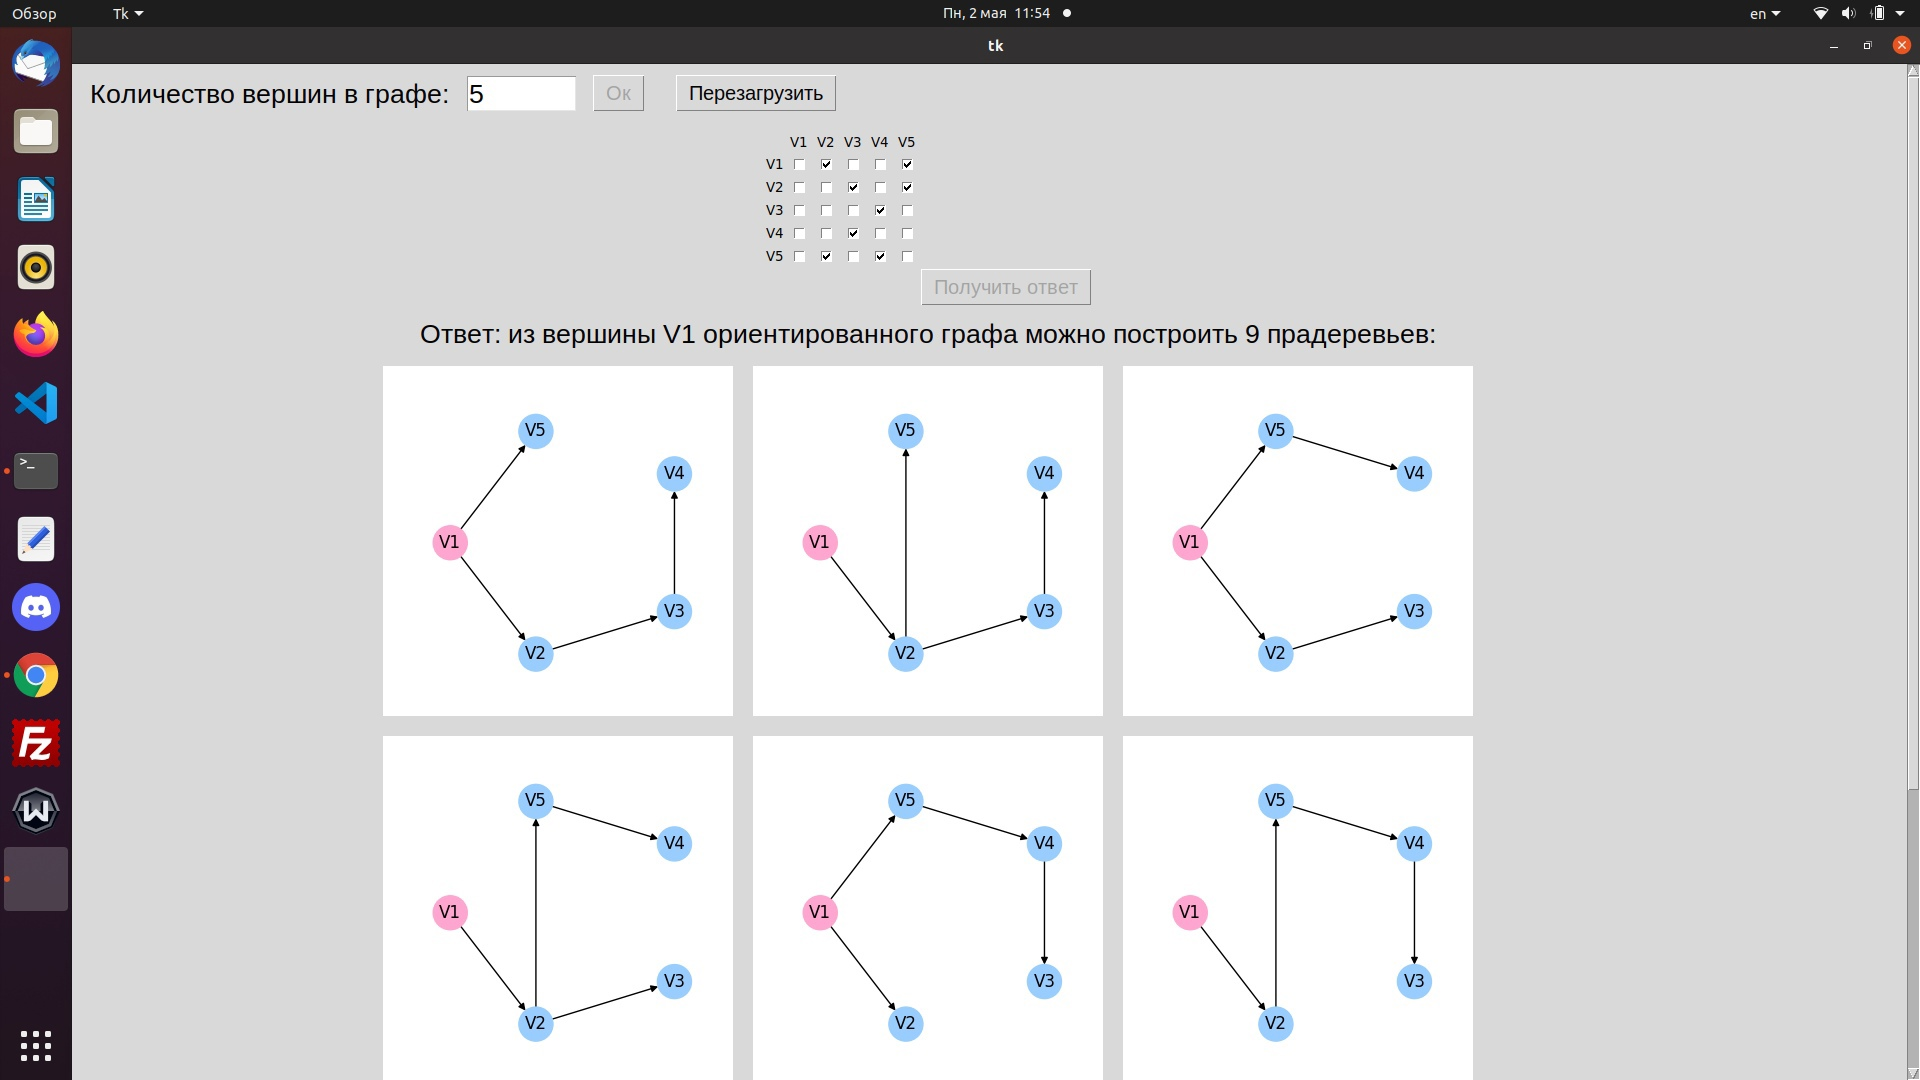
\includegraphics [scale=0.25]{ForDMreport.jpg}
\vspace{5mm}
\\
\noindent
\textbf{8. Прикладная задача} 
\begin{flushleft}
	Предположим у нас есть город столица некого окураг, помимо столицы в этом округе есть еще множество городов. Наша задача заключается в том, чтобы посчитать количество и вывести все возможные варианты того, каким образом можно проложить дороги от столицы до всех других городов.
\end{flushleft}
\end{document}